\hypertarget{intro}{%
\chapter{Introduction}\label{intro}}

In this \hb{class}, we will use the \R language, and the RStudio integrated development environment (IDE). Before the \hb{first meeting}, install the necessary software on your personal computer by executing the following instructions.

\hypertarget{installing-r-and-rstudio}{%
\section{Installing \R and Rstudio}\label{installing-r-and-rstudio}}

Go to the website of the Comprehensive R Archive Network (\url{https://cran.r-project.org/}) and download the latest version of \R for your operating system (Windows, MacOS, or Linux). As of \today, the latest version is 4.0.4. Follow the installation instructions.

Next, go the Rstudio download website
(\url{https://rstudio.com/products/rstudio/download/}) and get the Desktop version
(open source license). As of \today, the version is 1.4.1106. Follow the
installation instruction. An icon that looks like this:

\includegraphics[width=\textwidth,height=0.025\textheight]{images/RstudioLogo.png}
will be on your computer's desktop. Double-click on this icon to start the \R session. The Rstudio IDE will open, and look like this:

\begin{center}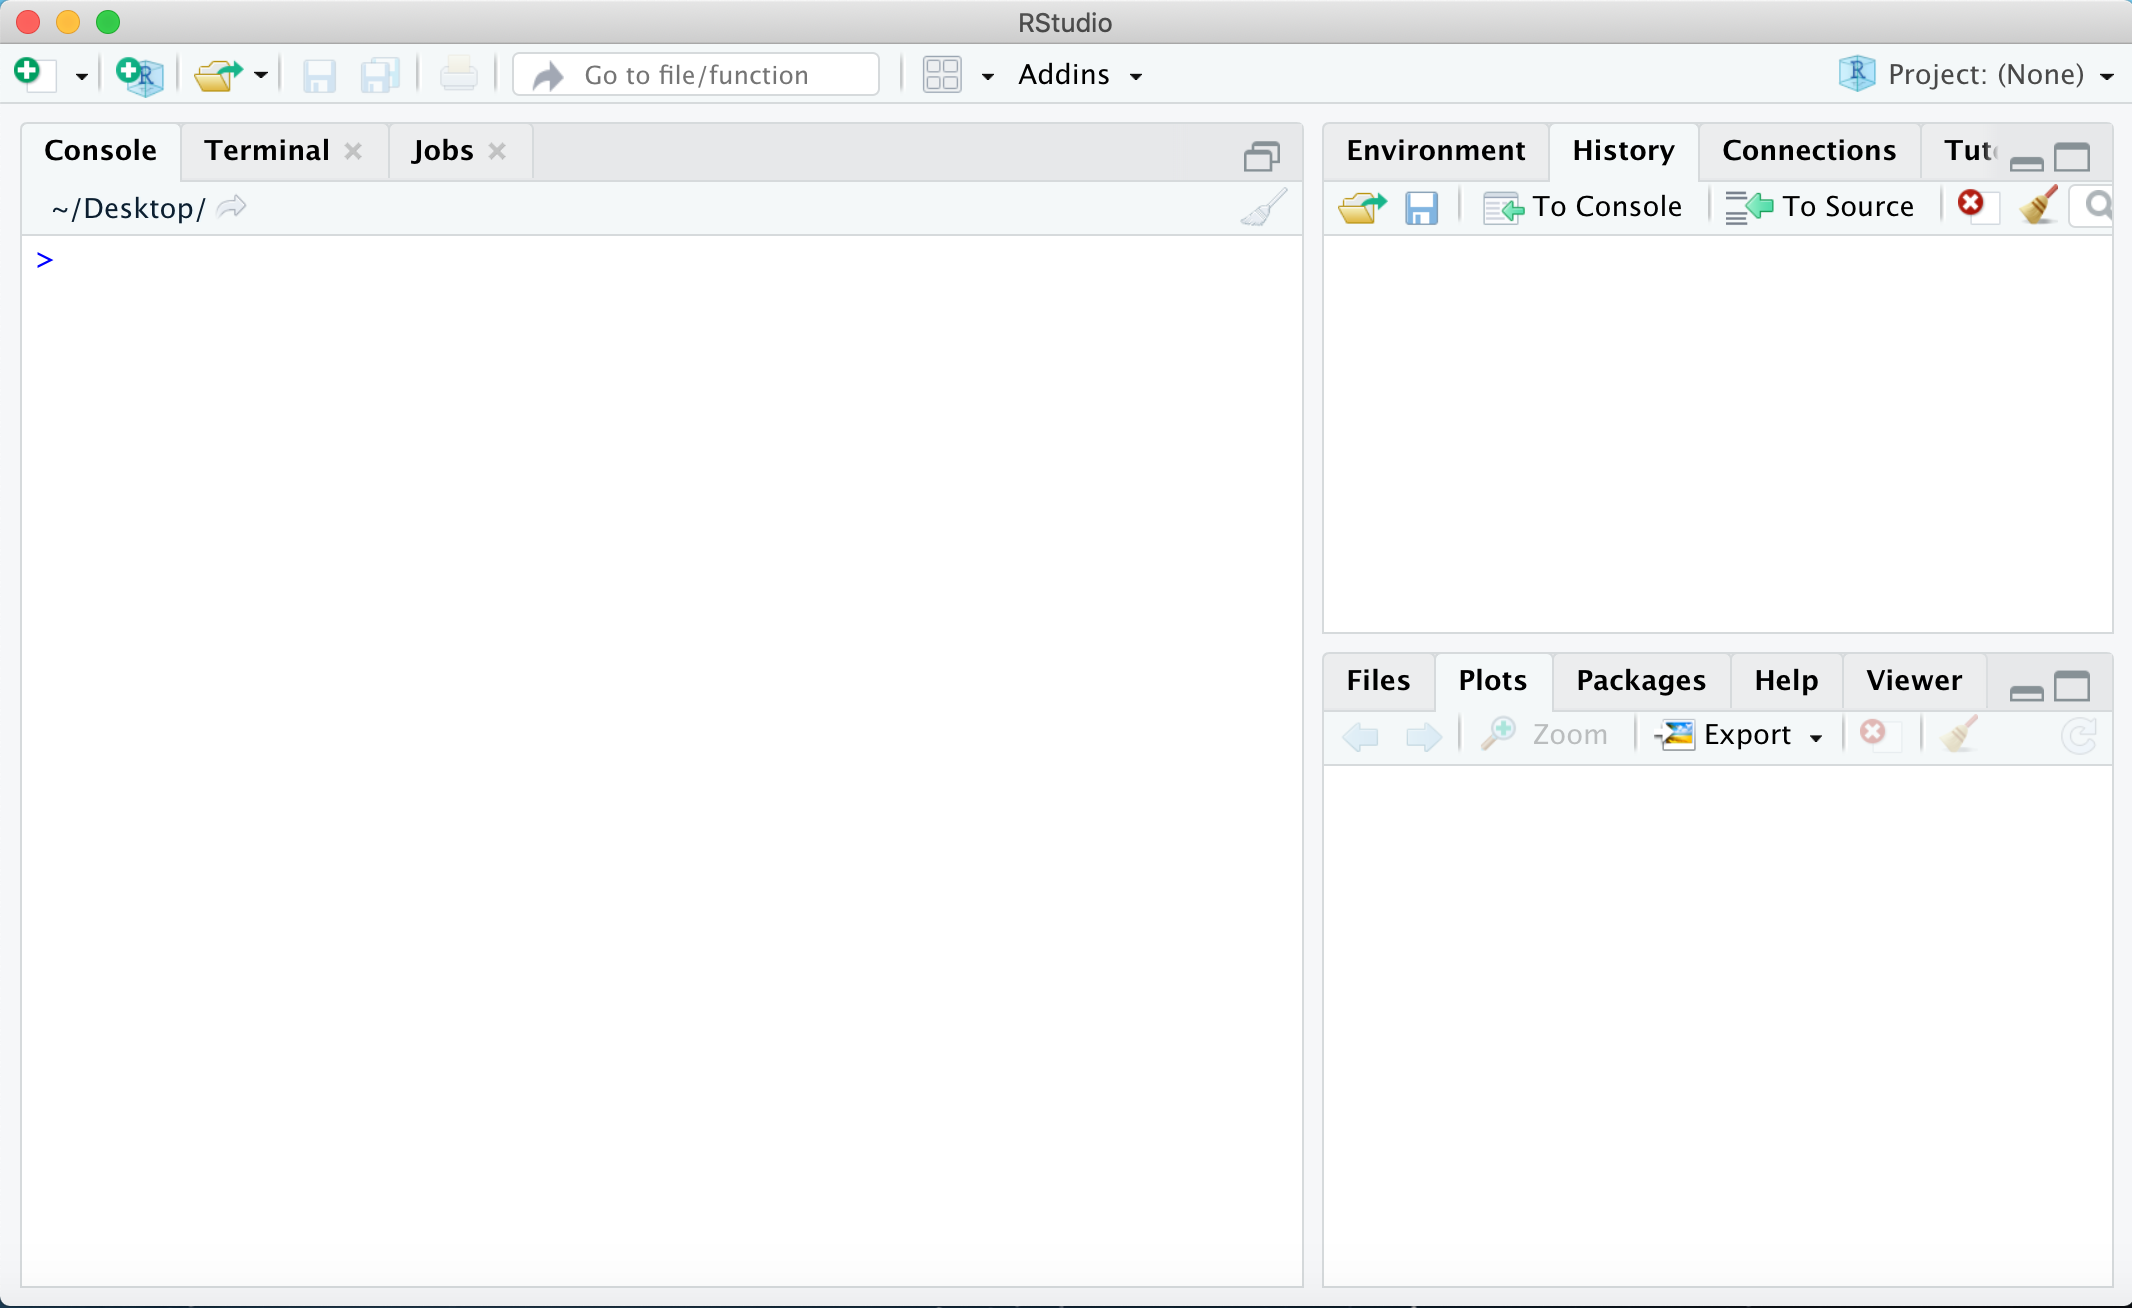
\includegraphics[width=0.8\linewidth]{images/RstudioMain} \end{center}

The left-hand side of the screen contains the Console tab. Notice the \(>\) sign (called the `prompt'). When you see this character, it means that \R is ready for the next command. Put the cursor there, and then type

\begin{verbatim}
2 + 2
\end{verbatim}

and hit Enter on the keyboard. You should get the following on the Console:

\begin{verbatim}
[1] 4
\end{verbatim}

Notice the top-right part of the Rstudio window. You should see an `Environment' and a `History' tab. Click on History. All your previous input appears there. Try entering another calculation or command and see that they appear in the session's history. For example, try entering the following

\begin{Shaded}
\begin{Highlighting}[]
\DecValTok{3} \SpecialCharTok{\^{}} \DecValTok{5}
\FunctionTok{date}\NormalTok{()}
\end{Highlighting}
\end{Shaded}

Click on the Environment tab. It should be empty when you start \R for the first time. In the Console, type

\begin{Shaded}
\begin{Highlighting}[]
\NormalTok{myFirstVariable }\OtherTok{\textless{}{-}} \FunctionTok{factorial}\NormalTok{(}\DecValTok{5}\NormalTok{)}
\end{Highlighting}
\end{Shaded}

Notice that nothing was printed in the Console, but the Environment tab now contains a table with one row, with `myFirstVariable' appearing in the cell on the left, and its value (120) on the right. Any object appearing in the Environment tab is available to you throughout your \R session, and you don't have to redefine or recalculate it. For example, you can try the following:

\begin{Shaded}
\begin{Highlighting}[]
\NormalTok{myFirstVariable}\SpecialCharTok{/}\DecValTok{6}
\end{Highlighting}
\end{Shaded}

The Console should now display 20.

The lower-right side of the IDE contains a file browser (the Files tab), information about installed packages (more about it later), and any plot generated during the \R session. It also contains a Help tab, to obtain information about built-in functions.

Finally, before we move on to the next section, in the Rstudio top menu, click on File, then on New File, and then on \R Script. Alternatively, you can click on little green `+' icon in the top-left part of the IDE. This will split the left side of the Rstudio IDE into two parts -- the lower part will contain the Console, and the top part will contain a tab labeled `Untitled1'. This is where you can enter \R code which you will save to a permanent file, and re-use later.
For example, enter the following in the blank space in the Untitled1 tab:

\begin{Shaded}
\begin{Highlighting}[]
\CommentTok{\# This is my first \R program}
\FunctionTok{cat}\NormalTok{(}\StringTok{\textquotesingle{}Hello, World!}\SpecialCharTok{\textbackslash{}n}\StringTok{\textquotesingle{}}\NormalTok{)}
\end{Highlighting}
\end{Shaded}

Then, from the main menu in Rstudio, click on File, then on Save, and in the `Save As' box enter FirstProgram.R and click the Save button.
Notice that the tab name is now FirstProgram.R.

In that part of the window, there should now be a small button called Source. Click on it. The program will be executed and the output will be shown in the Console. You can also execute individual lines in the source code. Just put the cursor anywhere in that line, and click on the Run button (which is near the Source button) or click Ctrl+Enter (or Command+Enter on a Mac). 

That's it. In the rest of these notes we will see more features of Rstudio, but you are now ready to start learning programming in R.


\section{Basic Operations in R}
\subsection{Some Useful Functions}
\R has many built-in functions, and many more in external packages. We will introduce them as we go, but let's get started with some basic ones.
The documentation on each function can be obtained by using \code{?func} or \code{help(func)} where \texttt{func} is some function. For example, to get the documentation about using the \code{help()} function, try the following:
\begin{knitrout}
\definecolor{shadecolor}{rgb}{0.969, 0.969, 0.969}\color{fgcolor}\begin{kframe}
\begin{alltt}
\hlkwd{help}\hlstd{(help)}
\hlopt{?}\hlstd{help}
\end{alltt}
\end{kframe}
\end{knitrout}

When we start an \R session, it's important to determine the `working directory'. This is the folder on our computer which \R will use to search for data or code files and save results. To find out which folder is currently used, we use the \code{getwd()} function
\begin{knitrout}
\definecolor{shadecolor}{rgb}{0.969, 0.969, 0.969}\color{fgcolor}\begin{kframe}
\begin{alltt}
\hlkwd{getwd}\hlstd{()}
\end{alltt}
\begin{verbatim}
[1] "/Users/runner/work/sids/sids/book/Rnw"
\end{verbatim}
\end{kframe}
\end{knitrout}

If we want (and we often will), we may change the working directory by using \code{setwd()}.  
\begin{knitrout}
\definecolor{shadecolor}{rgb}{0.969, 0.969, 0.969}\color{fgcolor}\begin{kframe}
\begin{alltt}
\hlkwd{setwd}\hlstd{(}\hlstr{"~/Desktop"}\hlstd{)}
\end{alltt}
\end{kframe}
\end{knitrout}
The \verb|~/| notation is a shortcut to your home directory. Using this shortcut is convenient because if you are using different computers or you share code with others, the home directory may be different on each computer.

Data is stored in variables. We can get the data from a file (Excel, comma-separated values, etc.), the Internet, or we can generate it ourselves. Let's start by generating some data.
The simplest function to create data is called \code{c()}, which stands for `combine'.
\begin{knitrout}
\definecolor{shadecolor}{rgb}{0.969, 0.969, 0.969}\color{fgcolor}\begin{kframe}
\begin{alltt}
\hlstd{(courseNames} \hlkwb{<-} \hlkwd{c}\hlstd{(}\hlstr{"Data Science"}\hlstd{,} \hlstr{"Statistics"}\hlstd{,} \hlstr{"Probability"}\hlstd{))}
\end{alltt}
\begin{verbatim}
[1] "Data Science" "Statistics"   "Probability" 
\end{verbatim}
\end{kframe}
\end{knitrout}
We created a variable called courseNames, and it contains three values. Note that we assigned the values into the variable by using the \verb|<-| operator. The parentheses around the whole statement cause the content of the variable to printed immediately to the console.
We can now do things with this variable. For example, we can check the variable type, using the \code{class()} function.
We can also get a bit more detailed information by checking its structure, using the \code{str()} function.
\begin{knitrout}
\definecolor{shadecolor}{rgb}{0.969, 0.969, 0.969}\color{fgcolor}\begin{kframe}
\begin{alltt}
\hlkwd{class}\hlstd{(courseNames)}
\end{alltt}
\begin{verbatim}
[1] "character"
\end{verbatim}
\begin{alltt}
\hlkwd{str}\hlstd{(courseNames)}
\end{alltt}
\begin{verbatim}
 chr [1:3] "Data Science" "Statistics" "Probability"
\end{verbatim}
\end{kframe}
\end{knitrout}
The variable is of class `character', and it is a vector with three values. 
We can check the number of elements in a vector by using the \code{length()} function:
\begin{knitrout}
\definecolor{shadecolor}{rgb}{0.969, 0.969, 0.969}\color{fgcolor}\begin{kframe}
\begin{alltt}
\hlkwd{length}\hlstd{(courseNames)}
\end{alltt}
\begin{verbatim}
[1] 3
\end{verbatim}
\end{kframe}
\end{knitrout}

Pick good variable names. They should describe the meaning of the value, yet be short enough to type. Variable names can only contain letters, numbers, the dot character, or the underline character. Variable names can only begin with either a letter, or a dot as long as it is not followed by a number. They should not be the same as an existing function name or other reserved words in the language (like `while', `if', `quit'.)

We can also generate variables which contain sequences of numbers. To do that, we use the \code{seq()} function. For example, we can create a variable which contains all the odd numbers between 1 and 20:
\begin{knitrout}
\definecolor{shadecolor}{rgb}{0.969, 0.969, 0.969}\color{fgcolor}\begin{kframe}
\begin{alltt}
\hlstd{(oddLT20} \hlkwb{<-} \hlkwd{seq}\hlstd{(}\hlnum{1}\hlstd{,}\hlnum{20}\hlstd{,}\hlkwc{by}\hlstd{=}\hlnum{2}\hlstd{))}
\end{alltt}
\begin{verbatim}
 [1]  1  3  5  7  9 11 13 15 17 19
\end{verbatim}
\begin{alltt}
\hlkwd{length}\hlstd{(oddLT20)}
\end{alltt}
\begin{verbatim}
[1] 10
\end{verbatim}
\end{kframe}
\end{knitrout}

To generate consecutive values, we can also use the colon operator:
\begin{knitrout}
\definecolor{shadecolor}{rgb}{0.969, 0.969, 0.969}\color{fgcolor}\begin{kframe}
\begin{alltt}
\hlstd{(firstThirteen} \hlkwb{<-} \hlnum{1}\hlopt{:}\hlnum{13}\hlstd{)}
\end{alltt}
\begin{verbatim}
 [1]  1  2  3  4  5  6  7  8  9 10 11 12 13
\end{verbatim}
\end{kframe}
\end{knitrout}

Another useful function to generate data is \code{rep()}, which replicates values.
We often have to generate a vector of ones or zeros, and we can do it like in the following example. We use this opportunitiy to also introduce the functions \code{sum()} and \code{cumsum()} (cumulative sum).
\begin{knitrout}
\definecolor{shadecolor}{rgb}{0.969, 0.969, 0.969}\color{fgcolor}\begin{kframe}
\begin{alltt}
\hlstd{(ones} \hlkwb{<-} \hlkwd{rep}\hlstd{(}\hlnum{1}\hlstd{,} \hlnum{10}\hlstd{))}
\end{alltt}
\begin{verbatim}
 [1] 1 1 1 1 1 1 1 1 1 1
\end{verbatim}
\begin{alltt}
\hlkwd{length}\hlstd{(ones)}
\end{alltt}
\begin{verbatim}
[1] 10
\end{verbatim}
\begin{alltt}
\hlkwd{sum}\hlstd{(ones)}
\end{alltt}
\begin{verbatim}
[1] 10
\end{verbatim}
\begin{alltt}
\hlkwd{cumsum}\hlstd{(ones)}
\end{alltt}
\begin{verbatim}
 [1]  1  2  3  4  5  6  7  8  9 10
\end{verbatim}
\end{kframe}
\end{knitrout}

There are also many functions to handle text. The \code{paste()} function attaches two strings of characters together. Note the usage of the collapse option (also called an `argument' of the function) in the second example:
\begin{knitrout}
\definecolor{shadecolor}{rgb}{0.969, 0.969, 0.969}\color{fgcolor}\begin{kframe}
\begin{alltt}
\hlkwd{paste}\hlstd{(courseNames)}
\end{alltt}
\begin{verbatim}
[1] "Data Science" "Statistics"   "Probability" 
\end{verbatim}
\begin{alltt}
\hlkwd{paste}\hlstd{(courseNames,} \hlkwc{collapse}\hlstd{=}\hlstr{", "}\hlstd{)}
\end{alltt}
\begin{verbatim}
[1] "Data Science, Statistics, Probability"
\end{verbatim}
\end{kframe}
\end{knitrout}

Let's combine what we've learned so far to create the 52 cards  in a standard deck, which includes four suits: Club, Diamond, Heart, and Spade:
\begin{knitrout}
\definecolor{shadecolor}{rgb}{0.969, 0.969, 0.969}\color{fgcolor}\begin{kframe}
\begin{alltt}
\hlstd{suits} \hlkwb{<-} \hlkwd{c}\hlstd{(}\hlkwd{rep}\hlstd{(}\hlstr{"C"}\hlstd{,}\hlnum{13}\hlstd{),} \hlkwd{rep}\hlstd{(}\hlstr{"D"}\hlstd{,}\hlnum{13}\hlstd{),} \hlkwd{rep}\hlstd{(}\hlstr{"H"}\hlstd{,}\hlnum{13}\hlstd{),} \hlkwd{rep}\hlstd{(}\hlstr{"S"}\hlstd{,}\hlnum{13}\hlstd{))}
\hlstd{(cards} \hlkwb{<-} \hlkwd{paste0}\hlstd{(suits,} \hlkwd{rep}\hlstd{(}\hlnum{1}\hlopt{:}\hlnum{13}\hlstd{,}\hlnum{4}\hlstd{)))}
\end{alltt}
\begin{verbatim}
 [1] "C1"  "C2"  "C3"  "C4"  "C5"  "C6"  "C7"  "C8"  "C9"  "C10" "C11" "C12"
[13] "C13" "D1"  "D2"  "D3"  "D4"  "D5"  "D6"  "D7"  "D8"  "D9"  "D10" "D11"
[25] "D12" "D13" "H1"  "H2"  "H3"  "H4"  "H5"  "H6"  "H7"  "H8"  "H9"  "H10"
[37] "H11" "H12" "H13" "S1"  "S2"  "S3"  "S4"  "S5"  "S6"  "S7"  "S8"  "S9" 
[49] "S10" "S11" "S12" "S13"
\end{verbatim}
\end{kframe}
\end{knitrout}
Note that \code{paste0()} is the same as \code{paste(..., collapse="")}.

Let's `deal' five cards to each player for a game of poker. We will use the \code{sample()} function.
\begin{knitrout}
\definecolor{shadecolor}{rgb}{0.969, 0.969, 0.969}\color{fgcolor}\begin{kframe}
\begin{alltt}
\hlkwd{set.seed}\hlstd{(}\hlnum{5252}\hlstd{)}
\hlstd{(pokerHand} \hlkwb{<-} \hlkwd{matrix}\hlstd{(}\hlkwd{sample}\hlstd{(cards,}\hlnum{20}\hlstd{,}\hlkwc{replace}\hlstd{=}\hlnum{FALSE}\hlstd{),} \hlkwc{nrow}\hlstd{=}\hlnum{5}\hlstd{,} \hlkwc{ncol}\hlstd{=}\hlnum{4}\hlstd{))}
\end{alltt}
\begin{verbatim}
     [,1]  [,2]  [,3]  [,4] 
[1,] "S8"  "S13" "S7"  "C4" 
[2,] "D8"  "C1"  "H6"  "H11"
[3,] "D4"  "C11" "S6"  "S11"
[4,] "D12" "C13" "S4"  "S1" 
[5,] "C6"  "S9"  "H12" "H9" 
\end{verbatim}
\end{kframe}
\end{knitrout}
The \code{sample()} function in this example is used to draw 20 cards at random from the deck, without replacement. Then, to divide it into four hands, we use the \code{matrix()} function, and specify the number of rows and the number of columns.

Check the class and the structure of the variable pokerHand, using the functions we've mentioned earlier.

We can save variables to a file in order to use them in a later session.
\begin{knitrout}
\definecolor{shadecolor}{rgb}{0.969, 0.969, 0.969}\color{fgcolor}\begin{kframe}
\begin{alltt}
\hlkwd{save}\hlstd{(pokerHand,} \hlkwc{file}\hlstd{=}\hlstr{"pokerHand.RData"}\hlstd{)}
\end{alltt}
\end{kframe}
\end{knitrout}
If we don't specify the complete path, the file will be stored in the current working directory. Recall that you can find out which directory is used with the \code{getwd()} function, and set it to another directory with \code{setwd()}.
Then, we may get the saved variables by using the following:
\begin{knitrout}
\definecolor{shadecolor}{rgb}{0.969, 0.969, 0.969}\color{fgcolor}\begin{kframe}
\begin{alltt}
\hlkwd{load}\hlstd{(}\hlstr{"pokerHand.RData"}\hlstd{)}
\end{alltt}
\end{kframe}
\end{knitrout}
After you use the \code{load()} function, the variable pokerHand will be available to use.

Variables which we do not save, will not be available once we terminate the current \R session. When we quit an \R session, we have an option to save the entire session's information. However, if there are variables, datasets, or functions which we have created and want to save, it's better to save them explicitly.

There are a few constants in \R, including the letters of the alphabet (upper- and lower-case), the month names, and the number $\pi$.
\begin{knitrout}
\definecolor{shadecolor}{rgb}{0.969, 0.969, 0.969}\color{fgcolor}\begin{kframe}
\begin{alltt}
\hlstd{LETTERS}
\end{alltt}
\begin{verbatim}
 [1] "A" "B" "C" "D" "E" "F" "G" "H" "I" "J" "K" "L" "M" "N" "O" "P" "Q" "R" "S"
[20] "T" "U" "V" "W" "X" "Y" "Z"
\end{verbatim}
\begin{alltt}
\hlstd{letters}
\end{alltt}
\begin{verbatim}
 [1] "a" "b" "c" "d" "e" "f" "g" "h" "i" "j" "k" "l" "m" "n" "o" "p" "q" "r" "s"
[20] "t" "u" "v" "w" "x" "y" "z"
\end{verbatim}
\begin{alltt}
\hlstd{month.abb}
\end{alltt}
\begin{verbatim}
 [1] "Jan" "Feb" "Mar" "Apr" "May" "Jun" "Jul" "Aug" "Sep" "Oct" "Nov" "Dec"
\end{verbatim}
\begin{alltt}
\hlstd{month.name}
\end{alltt}
\begin{verbatim}
 [1] "January"   "February"  "March"     "April"     "May"       "June"     
 [7] "July"      "August"    "September" "October"   "November"  "December" 
\end{verbatim}
\begin{alltt}
\hlstd{pi}
\end{alltt}
\begin{verbatim}
[1] 3.141593
\end{verbatim}
\end{kframe}
\end{knitrout}

The base distribution of \R is very comprehensive, but there are thousands of contributed packages which are written by \R users. We will use several such packages in the book, so let us see how to do it.
The package \pkg{lattice} provides `elegant high-level data visualization system with an emphasis on multivariate data'. To install the package, we use the \code{install.packages()} function.
\begin{knitrout}
\definecolor{shadecolor}{rgb}{0.969, 0.969, 0.969}\color{fgcolor}\begin{kframe}
\begin{alltt}
\hlkwd{install.packages}\hlstd{(}\hlstr{"lattice"}\hlstd{)}
\end{alltt}
\end{kframe}
\end{knitrout}
This has to be done just once. Occasionally, you may be prompted to install updates, which can also be done by using the \code{update.packages()} function.
To use the package, we need to load it, using the \code{library()} function. In the following example we use a built-in dataset of opera singers, and we plot their heights by their vocal parts.
\begin{knitrout}
\definecolor{shadecolor}{rgb}{0.969, 0.969, 0.969}\color{fgcolor}\begin{kframe}
\begin{alltt}
\hlkwd{library}\hlstd{(}\hlstr{"lattice"}\hlstd{)}
\hlkwd{bwplot}\hlstd{(voice.part} \hlopt{~} \hlstd{height,} \hlkwc{data}\hlstd{=singer,} \hlkwc{xlab}\hlstd{=}\hlstr{"Height (inches)"}\hlstd{)}
\end{alltt}
\end{kframe}\begin{figure}

{\centering 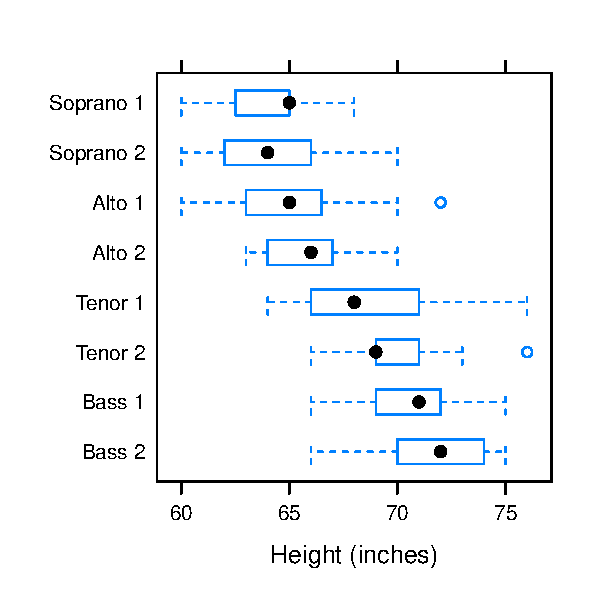
\includegraphics[width=\maxwidth]{figure/intro-pkg-1} 

}

\caption[Using the lattice package to create boxplots]{Using the lattice package to create boxplots}\label{fig:intro-pkg}
\end{figure}

\end{knitrout}


When you want to finish your session, just type \code{quit()}.



\subsection{Generating random numbers}
In this \hb{course}, much of the learning will be done by using simulated data, so let's start by learning how to generate data. The basic function to generate random data is \code{runif()} which is used to draw random numbers, uniformly between 0 and 1. In the following example we create 10,000 random draws from a uniform distribution, keep these numbers in a variable called simData, and plot a histogram to show the distribution of the data we have generated. The \code{set.seed()} function is used to ensure that every time we run this code, we will get the same set of random numbers. This is called \textit{reproducible code}. 
\begin{knitrout}
\definecolor{shadecolor}{rgb}{0.969, 0.969, 0.969}\color{fgcolor}\begin{kframe}
\begin{alltt}
\hlcom{# Generate 10,000 points from a uniform distribution}
\hlkwd{set.seed}\hlstd{(}\hlnum{210313}\hlstd{)}
\hlstd{n} \hlkwb{<-} \hlnum{10000}
\hlstd{simData} \hlkwb{<-} \hlkwd{runif}\hlstd{(n)}
\hlkwd{hist}\hlstd{(simData)}
\end{alltt}
\end{kframe}\begin{figure}

{\centering 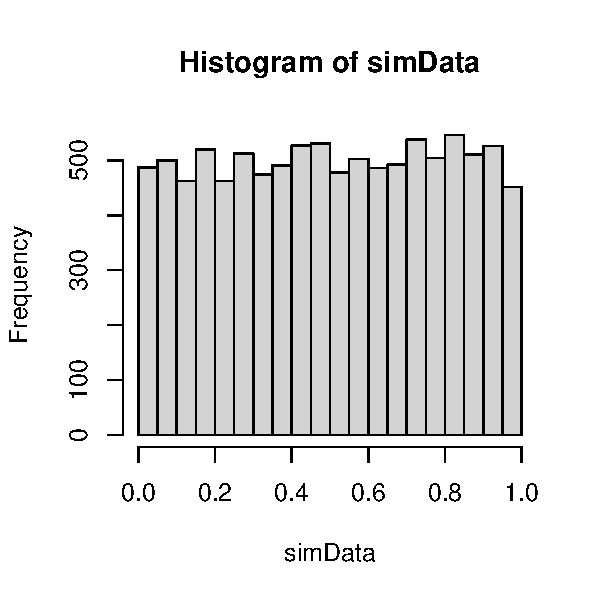
\includegraphics[width=\maxwidth]{figure/intro-runif-1} 

}

\caption[A histogram of 10,000 randomly drawn numbers from a standard uniform distribution]{A histogram of 10,000 randomly drawn numbers from a standard uniform distribution.}\label{fig:intro-runif}
\end{figure}

\end{knitrout}


From the range and the flatness of the histogram we can see that the generated data is indeed uniform on [0,1]. The \code{runif()} function can be used to draw random numbers uniformly on any finite interval. For example, if we want our random numbers to be in the interval [1,5] we will run the following code:

\begin{knitrout}
\definecolor{shadecolor}{rgb}{0.969, 0.969, 0.969}\color{fgcolor}\begin{kframe}
\begin{alltt}
\hlstd{n} \hlkwb{<-} \hlnum{10000}
\hlstd{simData} \hlkwb{<-} \hlkwd{runif}\hlstd{(n,} \hlkwc{min}\hlstd{=}\hlnum{1}\hlstd{,} \hlkwc{max}\hlstd{=}\hlnum{5}\hlstd{)}
\end{alltt}
\end{kframe}
\end{knitrout}

Try it, and draw the histogram as in the previous example. Try it with a fixed seed and verify that you get the same output each time. Then, run the code without a fixed seed and observe that you get a different distribution each time. Since the number of random draws is fairly large, the shape of the histogram will not change much.

From a random draw of a uniform distribution we can generate random numbers from other distributions. For example, we want to simulate (fair) coin flips, and count the number of Heads that we get. Let's say we want to simulate 200 coin tosses. We will draw 200 random numbers from a uniform distribution, and decide that we got Heads in the $i$-th toss if the $i$-the random number is less than 0.5, and Tails otherwise.
Try the following code multiple times (do not use \code{set.seed()}). What do you observe? We will discuss it further in a different \hb{lecture}.
\begin{knitrout}
\definecolor{shadecolor}{rgb}{0.969, 0.969, 0.969}\color{fgcolor}\begin{kframe}
\begin{alltt}
\hlcom{# Simulate 200 coin-flips, using the runif function:}
\hlstd{n.trials} \hlkwb{<-} \hlnum{200}
\hlkwd{cat}\hlstd{(}\hlstr{"Number of Heads is: "}\hlstd{,} \hlkwd{sum}\hlstd{(}\hlkwd{runif}\hlstd{(n.trials)} \hlopt{<} \hlnum{0.5}\hlstd{),} \hlstr{"\textbackslash{}n"}\hlstd{)}
\end{alltt}
\begin{verbatim}
Outout: Number of Heads is:  92
\end{verbatim}
\end{kframe}
\end{knitrout}


A few comments:
\begin{itemize}
\item A comment in \R starts with \#. Any text following the \# sign is considered user-documentation and is not executed by \R.
\item We have used the \code{cat()} function to print (concatenate) text to the console. Fixed text appears in double (or single) quotes, but the content of variables or output from \R functions should not be quoted. The \verb|\n| symbol tells \R to print a newline character at the end. Try to see what happens if you remove it.
\item The expression within the \code{sum()} function produces TRUE/FALSE (Boolean) values. First, we draw n.trials random numbers from a uniform distribution. Then, each one is compared with 0.5. If the value is less than 0.5, the returned value is TRUE. Otherwise, it's FALSE. This demonstrates one of \R's greatest features - allowing to run `vectorized' code. In one line, we generated 200 random numbers and compared each one to 0.5, and as a result, we got 200 Boolean values which we have added together (TRUE counts as 1, and FALSE counts as 0.) So, the result in the sum is the number of Heads in 200 tosses.
\end{itemize}

Statistical inference is based on a mental exercise in which we ask, if we could repeat the same experiment infinitely many times, what would we see? With simulations, we can get a good approximation. For example, the 200 coin-tosses experiment can be repeated, say, 100 times. One way is to use loops, like in the following example:
\begin{knitrout}
\definecolor{shadecolor}{rgb}{0.969, 0.969, 0.969}\color{fgcolor}\begin{kframe}
\begin{alltt}
\hlkwd{set.seed}\hlstd{(}\hlnum{442886}\hlstd{)}
\hlstd{n.trials} \hlkwb{<-} \hlnum{200}  \hlcom{# the number of coin-tosses in each experiment}
\hlstd{reps} \hlkwb{<-} \hlnum{100}  \hlcom{# the number of experiments}
\hlstd{Heads} \hlkwb{<-} \hlkwd{rep}\hlstd{(}\hlnum{0}\hlstd{, reps)}  \hlcom{# A vector to store the results (initialize with 0s)}
\hlkwa{for} \hlstd{(i} \hlkwa{in} \hlnum{1}\hlopt{:}\hlstd{reps) \{}
  \hlstd{Heads[i]} \hlkwb{<-} \hlkwd{sum}\hlstd{((}\hlkwd{runif}\hlstd{(n.trials)} \hlopt{<} \hlnum{0.5}\hlstd{))}
\hlstd{\}}
\hlkwd{hist}\hlstd{(Heads,} \hlkwc{breaks}\hlstd{=}\hlnum{20}\hlstd{)}
\end{alltt}
\end{kframe}\begin{figure}

{\centering 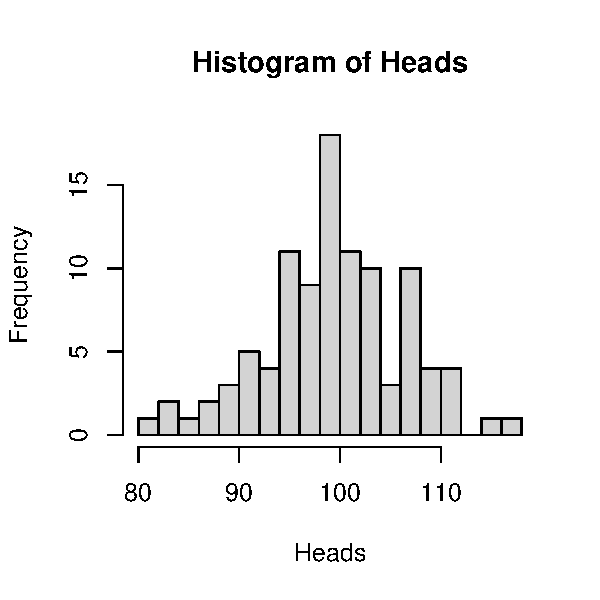
\includegraphics[width=\maxwidth]{figure/intro-heads2-1} 

}

\caption[A histogram of 100 experiments, from each we get the total number of Heads in 200 fair coin tosses]{A histogram of 100 experiments, from each we get the total number of Heads in 200 fair coin tosses.}\label{fig:intro-heads2}
\end{figure}

\end{knitrout}


We've used a \code{for()} loop, with an index variable called \texttt{i} which runs from 1 to 100. In each iteration we simulated n.trials=200 coin tosses, as before. The result from each iteration is stored in the $i$-th position in the vector we called Heads.

Using the uniform distribution, we have created a random draw from a different distribution, called the `binomial'. The mathematical notation is $Bin(N, p)$ where $N$ is the number of trials such that in each trial there can be exactly two outcomes (e.g., coin tosses), and $p$ is the probability of the first possible outcome (e.g., Head), and $1-p$ is the probability of the second possible outcome (e.g., Tail).
\R has a built-in function to generate random numbers from many different distributions, so the code above can be replaced by the following, which uses the \code{rbinom()} function:
\begin{knitrout}
\definecolor{shadecolor}{rgb}{0.969, 0.969, 0.969}\color{fgcolor}\begin{kframe}
\begin{alltt}
\hlkwd{set.seed}\hlstd{(}\hlnum{442886}\hlstd{)}
\hlstd{reps} \hlkwb{<-} \hlnum{100}
\hlstd{n.trials} \hlkwb{<-} \hlnum{200}
\hlstd{Heads} \hlkwb{<-} \hlkwd{rbinom}\hlstd{(reps, n.trials,} \hlnum{0.5}\hlstd{)}
\hlkwd{hist}\hlstd{(Heads,} \hlkwc{breaks}\hlstd{=}\hlnum{20}\hlstd{)}
\end{alltt}
\end{kframe}\begin{figure}

{\centering 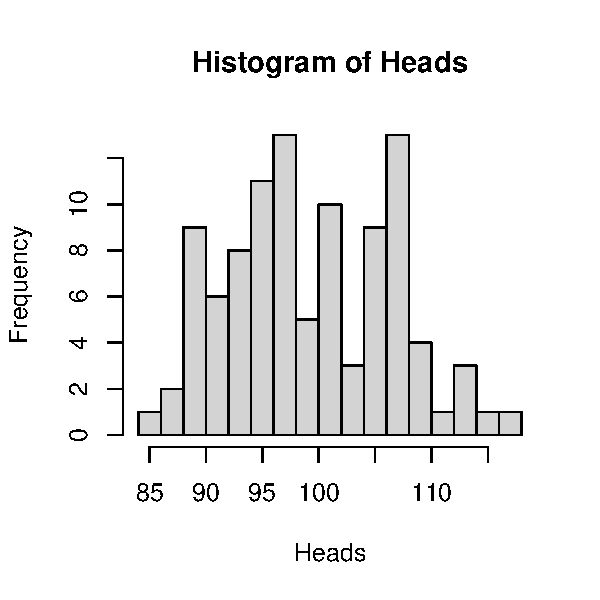
\includegraphics[width=\maxwidth]{figure/intro-binomial-1} 

}

\caption[A histogram of 100 binomial experiments, using rbinom() to simulate 200 fair coin tosses in each experiment]{A histogram of 100 binomial experiments, using rbinom() to simulate 200 fair coin tosses in each experiment.}\label{fig:intro-binomial}
\end{figure}

\end{knitrout}


Exercises:
\begin{enumerate}
\item Change the number of simulated coin-toss datasets (\texttt{reps}) to 1,000 and rerun the code. Then change it to 10,000 and run it again. What do you notice?
\item Change the probability of Heads to 0.2 and run the code again. Then, change it to 0.8. What do you observe?
\item Try other values of the number of trials and the probability of Heads.
\end{enumerate}




\subsection{Summary statistics}

We will introduce some statistical functions to summarize data. To demonstrate some of these functions, let's first generate some data:

\begin{knitrout}
\definecolor{shadecolor}{rgb}{0.969, 0.969, 0.969}\color{fgcolor}\begin{kframe}
\begin{alltt}
\hlstd{n} \hlkwb{<-} \hlnum{10000}
\hlstd{lambda} \hlkwb{<-} \hlnum{10}
\hlstd{x} \hlkwb{<-} \hlopt{-}\hlkwd{log}\hlstd{(}\hlkwd{runif}\hlstd{(n))}\hlopt{/}\hlstd{lambda}
\end{alltt}
\end{kframe}
\end{knitrout}

Note that in \R, the \code{log} function uses the natural logarithm by default. To use base 10 or base 2, use \code{log10} and \code{log2}, respectively. To specify the base, use the \code{base} argument. For example, try  \code{log(16, base=4)}.

The most commonly used one is the mean (a.k.a. the average), $\overline{x}$:\\
$$\overline{x}=\frac{x_1+\ldots+x_n}{n}\,.$$
Other ways to estimate some sort of `central tendency' of a distribution are:
 \begin{itemize}
 \item The trimmed mean, which is similar to the mean, except that the smallest and largest $p\cdot 100\%$  of the values are excluded from the computation. In our example, if we take $p=0.1$ with the simulated data, only 8,000 data points will be used in the calculation of the trimmed mean; 
 \item The median, which is a number (denoted here by $x_{0.5}$) such that half the data points are greater than $x_{0.5}$ and half are less than or equal to $x_{0.5}$. 
 \end{itemize}

Let's compute the sample's mean, trimmed mean, and median. Notice that  in this example the mean is greater than trimmed mean, which is greater than the median. In general, the mean is not a great estimate of the `center' of a non-symmetric distribution. We say that the mean is more `sensitive to extreme values' than the median.
\begin{knitrout}
\definecolor{shadecolor}{rgb}{0.969, 0.969, 0.969}\color{fgcolor}\begin{kframe}
\begin{alltt}
\hlkwd{mean}\hlstd{(x)}
\end{alltt}
\begin{verbatim}
Output: [1] 0.1007422
\end{verbatim}
\begin{alltt}
\hlkwd{mean}\hlstd{(x,} \hlkwc{trim}\hlstd{=}\hlnum{0.1}\hlstd{)}
\end{alltt}
\begin{verbatim}
Output: [1] 0.08366724
\end{verbatim}
\begin{alltt}
\hlkwd{median}\hlstd{(x)}
\end{alltt}
\begin{verbatim}
Output: [1] 0.07046186
\end{verbatim}
\end{kframe}
\end{knitrout}

The formula we used to generate the data is the probability function of the exponential distribution, with rate parameter $\lambda=10$. We denote it by $X\sim exp(\lambda)$. The exponential distribution is often used to model random waiting times, like the time between incoming text messages. We would usually generate it by using the \code{rexp()} function in \R.
Mathematical analysis of the distribution leads to the fact that the expected value of an exponential random variable with rate $\lambda$, is $1/\lambda$. We see that the theoretical expected value of our example is 0.1, and the sample mean is very close to 0.1. This is no coincidence - we will discuss it in  later chapter.


The distribution of \texttt{x} is shown below as a \textit{box-and-whisker plot} (or simply, boxplot). This is a very simple representation of numeric data, which is constructed by summarizing the data using a few numeric characteristics. The boxplot below is drawn horizontally, and the vertical grey line inside the box is the median. Similar to the median, we find the first quartile -- a point, $x_{0.25}$, such that 25\% of the values are less than $x_{0.25}$ and 75\% are greater than $x_{25}$; and the third quartile -- a point, $x_{0.75}$, such that 75\% of the values are less than $x_{0.75}$ and 25\% are greater than $x_{0.75}$. The first and third quartiles are the vertical edges of the box, also called the lower and upper hinges. So, the box represents 50\% of the data. The range between the first and third quartiles is called the \textit{Inter-Quartile Range}, or IQR, which is sometimes used to estimate the dispersion or spread of the data.
The `whiskers', which are the dashed grey lines, are constructed by adding 1.5$\cdot$IQR to each side of the box. If the result is smaller than the minimum value (or greater than the maximum), then the whisker only extends to the minimum (maximum). Points within the range between the two whiskers are not plotted individually, since their distribution is summarized succinctly by the box-and-whiskers plot. Points outside the range between the two whiskers are considered `outliers', or extreme values, and are shown explicitly. 

The plot was generated with the following code. Try it, and try changing some of the parameters to understand their role. We will cover the topic of visualization in a different chapter.

\begin{knitrout}
\definecolor{shadecolor}{rgb}{0.969, 0.969, 0.969}\color{fgcolor}\begin{kframe}
\begin{alltt}
\hlkwd{boxplot}\hlstd{(x,} \hlkwc{cex}\hlstd{=}\hlnum{0.5}\hlstd{,} \hlkwc{col}\hlstd{=}\hlnum{4}\hlstd{,}\hlkwc{border} \hlstd{=} \hlstr{"grey66"}\hlstd{,} \hlkwc{horizontal} \hlstd{= T,} \hlkwc{axes}\hlstd{=F,} \hlkwc{at}\hlstd{=}\hlnum{0.25}\hlstd{)}
\hlkwd{axis}\hlstd{(}\hlnum{1}\hlstd{,} \hlkwc{pos} \hlstd{=} \hlnum{0}\hlstd{)}
\hlkwd{points}\hlstd{(}\hlkwd{mean}\hlstd{(x),}\hlnum{0.25}\hlstd{,}\hlkwc{col}\hlstd{=}\hlnum{2}\hlstd{,} \hlkwc{pch}\hlstd{=}\hlnum{19}\hlstd{,} \hlkwc{cex}\hlstd{=}\hlnum{0.7}\hlstd{)}
\hlkwd{points}\hlstd{(}\hlkwd{mean}\hlstd{(x,} \hlkwc{trim}\hlstd{=}\hlnum{0.1}\hlstd{),}\hlnum{0.25}\hlstd{,} \hlkwc{col}\hlstd{=}\hlstr{"brown"}\hlstd{,} \hlkwc{pch}\hlstd{=}\hlnum{18}\hlstd{)}
\end{alltt}
\end{kframe}\begin{figure}

{\centering 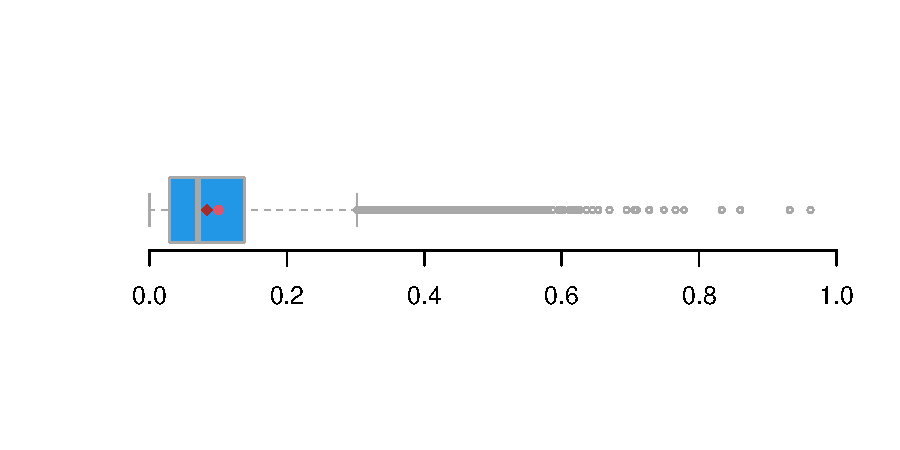
\includegraphics[width=\maxwidth]{figure/intro-boxplot-rexp-1} 

}

\caption[A boxplot]{A boxplot.}\label{fig:intro-boxplot-rexp}
\end{figure}

\end{knitrout}


A boxplot does not include the mean, or the trimmed mean, but we have added them here as a red circle and brown diamond, respectively, in order to show that they are different than the mean. The median is smaller than the mean in this case, so we say that the distribution is skewed to the left. The median does not depend on the scale of the data. It simply represents where half the data lies. 

A more detailed summary of a sample can be obtained by calculating its quantiles. In the boxplot, only three quantiles (also called percentiles) are shown. We can show the quintiles (20, 40, 60, 80 percentiles), or deciles (10, 20,\ldots, 90 percentiles) by using the \code{quantile()} function.

\begin{knitrout}
\definecolor{shadecolor}{rgb}{0.969, 0.969, 0.969}\color{fgcolor}\begin{kframe}
\begin{alltt}
\hlkwd{hist}\hlstd{(x,} \hlkwc{breaks}\hlstd{=}\hlnum{50}\hlstd{,} \hlkwc{border}\hlstd{=}\hlstr{"white"}\hlstd{,} \hlkwc{col}\hlstd{=}\hlstr{"lightblue"}\hlstd{,} \hlkwc{freq}\hlstd{=}\hlnum{FALSE}\hlstd{,} \hlkwc{xlim}\hlstd{=}\hlkwd{c}\hlstd{(}\hlnum{0}\hlstd{,}\hlnum{0.6}\hlstd{))}
\hlstd{deciles} \hlkwb{<-} \hlkwd{quantile}\hlstd{(x,} \hlkwc{probs}\hlstd{=}\hlkwd{seq}\hlstd{(}\hlnum{0.1}\hlstd{,}\hlnum{0.9}\hlstd{,}\hlkwc{by}\hlstd{=}\hlnum{0.1}\hlstd{))}
\hlkwd{abline}\hlstd{(}\hlkwc{v}\hlstd{=deciles,} \hlkwc{lty}\hlstd{=}\hlnum{2}\hlstd{,} \hlkwc{col}\hlstd{=}\hlstr{"purple"}\hlstd{,} \hlkwc{lwd}\hlstd{=}\hlnum{2}\hlstd{)}
\hlkwd{text}\hlstd{(deciles,} \hlkwd{dexp}\hlstd{(deciles,} \hlnum{10}\hlstd{),} \hlkwd{paste0}\hlstd{(}\hlkwd{seq}\hlstd{(}\hlnum{10}\hlstd{,}\hlnum{90}\hlstd{,}\hlkwc{by}\hlstd{=}\hlnum{10}\hlstd{),}\hlstr{"%"}\hlstd{),} \hlkwc{cex}\hlstd{=}\hlnum{0.7}\hlstd{,} \hlkwc{col}\hlstd{=}\hlstr{"orange"}\hlstd{)}
\end{alltt}
\end{kframe}\begin{figure}

{\centering 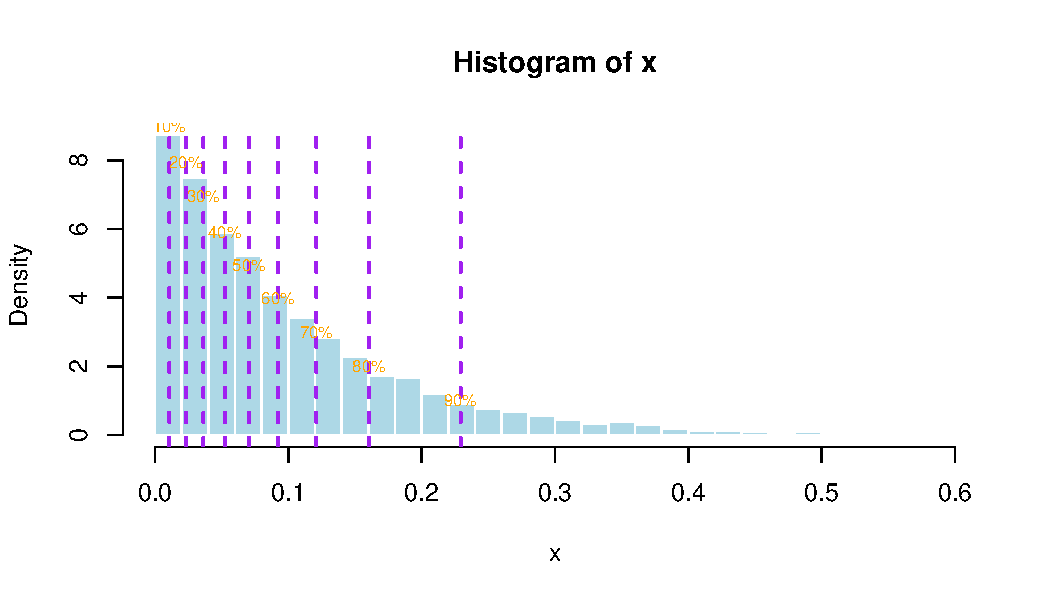
\includegraphics[width=\maxwidth]{figure/intro-quantile-rexp-1} 

}

\caption[A histogram of a sample from an exponential distribution, with the 10, 20, 30,..]{A histogram of a sample from an exponential distribution, with the 10, 20, 30,... percentiles}\label{fig:intro-quantile-rexp}
\end{figure}

\end{knitrout}


In addition to sample statistics which summarize some notion of the center of the distribution, we are often interested in estimating the dispersion of the data. The most commonly used measures of dispersion are the variance, and its square root - the standard deviation. The variance is defined as follows

$$Var(X)=\frac{(x_1-\mu)^2+\ldots+(x_n-\mu)^2}{n}$$
 where $\mu$ is the mean of the distribution of $X$. In words, the variance is the average squared deviation from the mean.
Notice that in \R the variance is computed with n-1 in the denominator (with n-1 we get an `unbiased estimator' for the true variance).

The corresponding functions in \R are \code{var()} and \code{sd()}. In the following code we also demonstrate the \code{IQR()} function.
\begin{knitrout}
\definecolor{shadecolor}{rgb}{0.969, 0.969, 0.969}\color{fgcolor}\begin{kframe}
\begin{alltt}
\hlkwd{var}\hlstd{(x)}
\end{alltt}
\begin{verbatim}
Output: [1] 0.01010772
\end{verbatim}
\begin{alltt}
\hlkwd{sd}\hlstd{(x)} \hlcom{# note that sd(x) is sqrt(sd(x))}
\end{alltt}
\begin{verbatim}
Output: [1] 0.1005371
\end{verbatim}
\begin{alltt}
\hlkwd{IQR}\hlstd{(x)}
\end{alltt}
\begin{verbatim}
Output: [1] 0.1091089
\end{verbatim}
\end{kframe}
\end{knitrout}

We will see in subsequent chapters that the normal distribution plays a major role in statistics. It is defined by a probability density function, with two parameters -- $\mu$ and $\sigma^2$:
$$\phi(x; \mu,\sigma^2)=\frac{1}{\sqrt{2\pi\sigma^2}}\exp\left[-\frac{(x-\mu)^2}{2\sigma^2}\right]\,.$$
It is symmetric, `bell-shaped', and centered around the mean, $\mu$, as shown in the following plot. The blue histogram is generated by the \code{rnorm()} function, using $\mu=2.5$ and $\sigma^2=0.25$. The orange curve shows the function $\phi$, by using the \code{dnorm()} function (to obtain the density of $x$).
\begin{knitrout}
\definecolor{shadecolor}{rgb}{0.969, 0.969, 0.969}\color{fgcolor}\begin{kframe}
\begin{alltt}
\hlstd{x} \hlkwb{<-} \hlkwd{rnorm}\hlstd{(}\hlnum{10000}\hlstd{,} \hlkwc{mean}\hlstd{=}\hlnum{2.5}\hlstd{,} \hlkwc{sd}\hlstd{=}\hlnum{0.5}\hlstd{)}
\hlkwd{hist}\hlstd{(x,} \hlkwc{breaks}\hlstd{=}\hlnum{30}\hlstd{,} \hlkwc{border}\hlstd{=}\hlstr{"white"}\hlstd{,} \hlkwc{col}\hlstd{=}\hlstr{"navyblue"}\hlstd{,} \hlkwc{freq}\hlstd{=}\hlnum{FALSE}\hlstd{)}
\hlstd{xs} \hlkwb{<-} \hlkwd{seq} \hlstd{(}\hlnum{0}\hlstd{,}\hlnum{5}\hlstd{,} \hlkwc{length}\hlstd{=}\hlnum{500}\hlstd{)}
\hlkwd{lines}\hlstd{(xs,} \hlkwd{dnorm}\hlstd{(xs,}\hlnum{2.5}\hlstd{,} \hlnum{0.5}\hlstd{),} \hlkwc{col}\hlstd{=}\hlstr{"orange"}\hlstd{,} \hlkwc{lwd}\hlstd{=}\hlnum{3}\hlstd{)}
\end{alltt}
\end{kframe}\begin{figure}

{\centering 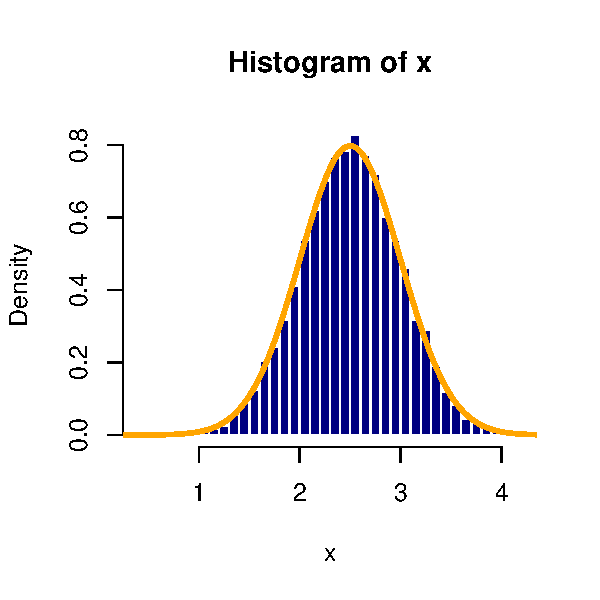
\includegraphics[width=\maxwidth]{figure/intro-rnorm1-1} 

}

\caption[A histogram of a sample from an normal distribution, with mean=2.5 and variance=0.25]{A histogram of a sample from an normal distribution, with mean=2.5 and variance=0.25}\label{fig:intro-rnorm1}
\end{figure}

\end{knitrout}

We can obtained more detailed summaries about the sample, by using the functions \code{summary()} and \code{describe()} (the latter is from the psych package, and provides more details.)

\begin{knitrout}
\definecolor{shadecolor}{rgb}{0.969, 0.969, 0.969}\color{fgcolor}\begin{kframe}
\begin{alltt}
\hlkwd{print}\hlstd{(}\hlkwd{summary}\hlstd{(x))}
\end{alltt}
\begin{verbatim}
Output:    Min. 1st Qu.  Median    Mean 3rd Qu.    Max. 
Output:  0.4667  2.1731  2.5068  2.5043  2.8377  4.1818
\end{verbatim}
\begin{alltt}
\hlkwd{print}\hlstd{(psych}\hlopt{::}\hlkwd{describe}\hlstd{(x))}
\end{alltt}
\begin{verbatim}
Output:    vars     n mean  sd median trimmed  mad  min  max range  skew kurtosis se
Output: X1    1 10000  2.5 0.5   2.51    2.51 0.49 0.47 4.18  3.72 -0.03     0.05  0
\end{verbatim}
\end{kframe}
\end{knitrout}

\code{summary()}  gives the minimum, maximum, the 25th, 50th, and 75th percentiles, as well as the mean of the sample. \code{psych::describe()} also gives the sample size, the standard deviation, the trimmed mean, the mean absolute deviation (mad), the range (maximum minus minimum), the skewness, and the kurtosis \hb{will we use the kurtosis later? If so, we should add a ref.}.

We conclude this chapter with some functions which can be used to summarize discrete (categorical) data, where the mean, variance, quantiles, etc. are not applicable. We will revisit the topic of summarizing data in the chapter on \hb{visualization}.

To simulate categorical data we can use the \code{rmultinom()} function, which simulates putting $N$ objects in $K$ bins with given probabilities. Another possibility is to use \code{cut()} function which divides a range of number into discrete ranges and creates discrete categories in a factor variable.
For example, suppose there is a town with three hotels (Motel 6, Best Western,  and Hilton) with 400, 300, and 300 rooms, and one auto rental company with only two makes of cars (700 Honda, and 300 Teslas). In the following code we simulate the allocation of 100 visitors to hotels and cars. We use the \code{table()} function to show the counts by hotel, by car, and by both. 

\begin{knitrout}
\definecolor{shadecolor}{rgb}{0.969, 0.969, 0.969}\color{fgcolor}\begin{kframe}
\begin{alltt}
\hlstd{hotelrooms} \hlkwb{<-} \hlkwd{cut}\hlstd{(}\hlkwd{runif}\hlstd{(}\hlnum{100}\hlstd{),}\hlkwc{breaks} \hlstd{=} \hlkwd{c}\hlstd{(}\hlnum{0}\hlstd{,}\hlnum{0.4}\hlstd{,}\hlnum{0.7}\hlstd{,}\hlnum{1}\hlstd{),} \hlkwc{include.lowest} \hlstd{=} \hlnum{TRUE}\hlstd{)}
\hlkwd{levels}\hlstd{(hotelrooms)} \hlkwb{<-} \hlkwd{c}\hlstd{(}\hlstr{"Motel 6"}\hlstd{,} \hlstr{"Best Western"}\hlstd{,} \hlstr{"Hilton"}\hlstd{)}
\hlstd{autorental} \hlkwb{<-} \hlkwd{cut}\hlstd{(}\hlkwd{runif}\hlstd{(}\hlnum{100}\hlstd{),}\hlkwc{breaks} \hlstd{=} \hlkwd{c}\hlstd{(}\hlnum{0}\hlstd{,}\hlnum{0.7}\hlstd{,}\hlnum{1}\hlstd{),} \hlkwc{include.lowest} \hlstd{=} \hlnum{TRUE}\hlstd{)}
\hlkwd{levels}\hlstd{(autorental)} \hlkwb{<-} \hlkwd{c}\hlstd{(}\hlstr{"Honda"}\hlstd{,} \hlstr{"Tesla"}\hlstd{)}
\hlstd{(hoteltbl} \hlkwb{<-} \hlkwd{table}\hlstd{(hotelrooms))}
\end{alltt}
\begin{verbatim}
Output: hotelrooms
Output:      Motel 6 Best Western       Hilton 
Output:           45           27           28
\end{verbatim}
\begin{alltt}
\hlstd{(autotbl} \hlkwb{<-} \hlkwd{table}\hlstd{(autorental))}
\end{alltt}
\begin{verbatim}
Output: autorental
Output: Honda Tesla 
Output:    69    31
\end{verbatim}
\begin{alltt}
\hlkwd{table}\hlstd{(hotelrooms, autorental)}
\end{alltt}
\begin{verbatim}
Output:               autorental
Output: hotelrooms     Honda Tesla
Output:   Motel 6         27    18
Output:   Best Western    21     6
Output:   Hilton          21     7
\end{verbatim}
\end{kframe}
\end{knitrout}

We can use the \code{max()} and \code{which.max()} functions to find the mode of the data (the most frequent value).

\begin{knitrout}
\definecolor{shadecolor}{rgb}{0.969, 0.969, 0.969}\color{fgcolor}\begin{kframe}
\begin{alltt}
\hlkwd{cat}\hlstd{(}\hlkwd{levels}\hlstd{(hotelrooms)[}\hlkwd{which.max}\hlstd{(hoteltbl)],}\hlstr{":"}\hlstd{,} \hlkwd{max}\hlstd{(hoteltbl),}\hlstr{"\textbackslash{}n"}\hlstd{)}
\end{alltt}
\begin{verbatim}
Output: Motel 6 : 45
\end{verbatim}
\begin{alltt}
\hlkwd{cat}\hlstd{(}\hlkwd{levels}\hlstd{(autorental)[}\hlkwd{which.max}\hlstd{(autotbl)],}\hlstr{":"}\hlstd{,} \hlkwd{max}\hlstd{(autotbl),}\hlstr{"\textbackslash{}n"}\hlstd{)}
\end{alltt}
\begin{verbatim}
Output: Honda : 69
\end{verbatim}
\end{kframe}
\end{knitrout}

%matrices
% in a chapter on visualization:
%.  more distributions - Poisson, beta, gamma, lognormal
%.  density plot
%.  ecdf
%.  Q-Q plot
%.  scatterplot

